\section{Эмпирическая функция распределения}

Пусть дана случайная выборка размера $n$ из распределения вероятностей $F$
\begin{equation}
    F\rightarrow(x_1,x_2,\cdots,x_n),
\end{equation}
тогда эмпирическая функция распределения  $F$ определяется как дискретное распределение, которое ставит вероятность $1 / n$ на каждое значение $x_i$, $i = 1, 2, \cdots, n$. Другими словами, $F$ присваивает множеству $A$ в пространстве выборок $x$ его эмпирическую вероятность 
\begin{equation}
    \widehat{Prob}\{A\}=\#\{x_i\in A\}/n,
\end{equation}
это доля наблюдаемой выборки $x = (x_1, x_2,\cdots, x_n)$, встречающейся в A. Мы также будем писать $Prob_{\hat F}\{A\}$ для обозначения (4.2). Символ в шляпе <<$\wedge$>> всегда указывает на величины, рассчитанные на основе наблюдаемых данных. 
\newline

\noindent
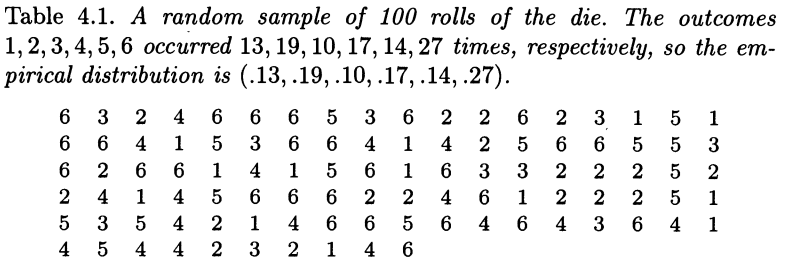
\includegraphics[width=\linewidth]{3/t41.png}
\newline

Рассмотрим выборку юридических вузов размером $n = 15$, показанную в Таблице 3.1 и на правой панели Рисунка 3.1. Эмпирическое распределение $F$ ставит вероятность $1/15$ для каждой из 15 точек данных. Пять из 15 точек лежат в наборе $A = \{(y, z): 0 <y <600,0 <z <3.00\}$, поэтому $\widehat{Prob}\{A\} = 5/15 = 0.333$. Обратите внимание, что мы получаем другую эмпирическую вероятность для набора $\{0 <y <600,0 <z \le 3.00\}$, поскольку одна из 15 точек данных имеет $GPA = 3.00$, $LSAT < 600$. 

Таблица 4.1 показывает случайную выборку из $n = 100$ бросков кубика: $x_1 = 6, x_2 = 3, x_3 = 2,\cdots, x_{100} = 6$. Эмпирическое распределение $F$ ставит вероятность $1/100$ для каждого из 100 исходов. В подобных случаях, когда есть повторяющиеся значения, мы можем более экономично выразить $F$ как вектор наблюдаемых частот $\hat f_k$, $k=1,2,\cdots,6$
\begin{equation}
    \hat f_k = \#\{x_i=k\}/n.
\end{equation}
Для данных в таблице 4.1 $\hat F= (0.13, 0.19, 0.10, 0.17, 0.14, 0.27)$.

Эмпирическое распределение -- это список значений, принимаемых выборкой $x = (x_1, x_2, \cdots, x_n)$, вместе с долей случаев, когда каждое значение встречается. Часто каждое значение, встречающееся в выборке, появляется только один раз, как в случае с данными юридических школ. Повторения, как и в случае с кубиком таблицы 4.1, позволяют сократить список. В любом случае каждой из $n$ точек данных $x_i$ приписывается вероятность $1 / n$ эмпирическим распределением. 

Очевидно ли, что мы не потеряли информацию при переходе от полного набора данных $(x_1, x_2,\cdots, x_{100})$ в таблице 4.1 к сокращенному представлению в терминах частот? Нет, но это правда. Можно доказать, что вектор наблюдаемых частот $\hat F = (\hat f_1, \hat f_2, \cdots)$ является достаточной статистикой для истинного распределения $F = (f_1, f_2, \cdots)$. Это означает, что вся информация о $F$, содержащаяся в $\mathbf{x}$, также содержится в $\hat F$. 
\newline

\noindent
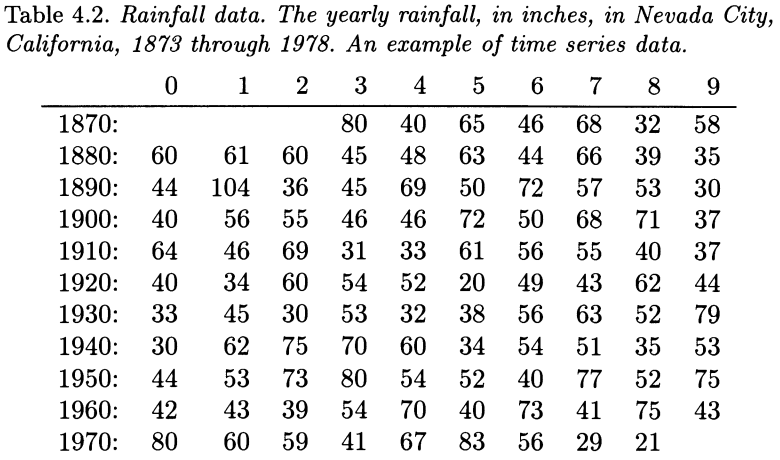
\includegraphics[width=\linewidth]{3/t42.png}
\newline

Теорема достаточности предполагает, что данные были сгенерированы случайной выборкой из некоторого распределения $F$. Это, конечно, не всегда верно. Например, данные о мышах в Таблице 2.1 включают два распределения вероятностей, одно для лечения и одно для контроля. В таблице 4.2 показан временной ряд из 106 чисел: годовое количество осадков в Невада-Сити, Калифорния, с 1873 по 1978 год. Мы могли бы вычислить эмпирическое распределение $F$ для этого набора данных, но оно не будет включать никакой информации временного ряда, например, если большие числа следуют за большими числами. На данный момент мы ограничиваем внимание данными, полученными путем случайной выборки из одного распределения, так называемой ситуации с одной выборкой. Это не так строго, как кажется. Например, в примере с данными о мышах мы можем применить результаты по одной выборке отдельно к экспериментальной и контрольной популяциям. 

При применении статистической теории к реальным задачам ответы на интересующие вопросы обычно формулируются в терминах вероятностных распределений. Мы можем спросить, справедлива ли матрица, дающая данные в Таблице 4.1. Это эквивалентно вопросу, равно ли распределение вероятностей $F$ кубика $(1/6, 1/6, 1/6, 1/6, 1/6, 1/6)$. В примере с юридической школой вопрос может заключаться в том, насколько коррелируют LSAT и GPA. В терминах $F$, распределение $x = (y, z) = (LSAT, GPA)$, это вопрос о значении коэффициента корреляции совокупности
\begin{equation}
    corr(y,z)=\frac{\sum_{j=1}^{82}(Y_j-\mu_y)(Z_j-\mu_z)}{[\sum_{j=1}^{82}(Y_j-\mu_y)^2\sum_{j=1}^{82}(Z_j-\mu_z)^2]^\frac{1}{2}},
\end{equation}
где $(Y_j, Z_j)$ -- j-я точка в популяции юридических школ $\mathbf{X}$, а $\mu_y = \sum_{j=1}^{82} Y_j / 82$, $\mu_z = \sum_{j=1}^{82} Z_j / 82$.

Когда распределение вероятностей $F$ известно (т.е. когда у нас есть полная совокупность $\mathbf{X}$), ответы на такие вопросы требуют не более чем арифметических операций. Для совокупности юридических школ перепись в таблице 3.2 дает $\mu_y = 597.5$, $\mu_z = 3.13$ и 
\begin{equation}
    corr(y,z)=0.761.
\end{equation}
Это первоначальное определение «статистики». Обычно у нас нет генеральной совокупности. Поэтому нам нужен статистический вывод, более современная статистическая теория для вывода свойств $F$ из случайной выборки $\mathbf{x}$. 

Если бы у нас была только выборка юридических школ размером 15, таблица 3.1, мы могли бы оценить $corr (y, z)$ с помощью коэффициента корреляции выборки 
\begin{equation}
    \widehat{corr}(y,z)=\frac{\sum_{j=1}^{15}(y_j-\hat\mu_y)(z_j-\hat\mu_z)}{[\sum_{j=1}^{15}(y_j-\hat\mu_y)^2\sum_{j=1}^{15}(z_j-\hat\mu_z)^2]^\frac{1}{2}},
\end{equation}
где $(y_j, z_j)$ - j-я точка в таблице 3.1, $j = 1, 2, \cdots, 15$ и $\hat\mu_y = \sum_{j=1}^{15}y_j/15$, $\hat\mu_z = \sum_{j=1}^{15}z_j / 15$. Таблица 3.1 дает $\mu_y = 600.3$, $\mu_z = 3.09$ и 
\begin{equation}
    \widehat{corr}(y,z)=0.776.
\end{equation}

Вот еще один пример оценки плагина. Предположим, нас интересует оценка вероятности того, что результат LSAT превышает 600, то есть 
\begin{equation}
    \theta=\frac{1}{82}\sum_1^{82}I_{\{Y_i>600\}}.
\end{equation}
Поскольку 39 из 82 баллов LSAT превышают 600, $\theta = 39/82 = 0.48$. Плагин оценка $\theta$ доли баллов LSAT, превышающих 600, равна 
\begin{equation}
    \hat\theta=\frac{1}{15}\sum_1^{15}I_{\{y_i>600\}}.
\end{equation}
Шесть из 15 баллов LSAT превышают 600, поэтому $\hat\theta = 6/15 = 0.4$. 

Для кубика в Таблице 4.1 у нас нет данных переписи, а есть только выборка $\mathbf{x}$, поэтому на любые вопросы о справедливости кубика необходимо отвечать, исходя из эмпирических частот
\begin{equation}
    \hat F=(\hat f_1, \hat f_2,\cdots,\hat f_6)=(0.13,0.19,0.10,0.17,0.14,0.27).
\end{equation}

Обсуждения статистического вывода сформулированы в терминах параметров и статистики. Параметр -- это функция распределения вероятностей $F$. Статистика -- это функция выборки $\mathbf{x}$. Таким образом, $corr (y, z)$, (4.4), является параметром $F$, а $\widehat{corr} (y, z)$, (4.6), является статистикой, основанной на $\mathbf{x}$. Точно так же $f_k$ -- это параметр $F$, а $\hat f_k$ -- статистика, $k = 1, 2, 3, \cdots, 6$.

Иногда мы будем писать параметры напрямую как функции от $F$, например
\begin{equation}
    \theta=t(F).
\end{equation}
Это обозначение подчеркивает, что значение параметра $\theta$ получается путем применения некоторой процедуры численной оценки $t(\cdot)$ к функции распределения $F$. Например, если $F$ -- это распределение вероятностей на действительной прямой, математическое ожидание можно представить как параметр 
\begin{equation}
    \theta=t(F)=E_F(x).
\end{equation}
Здесь $t(F)$ или $\theta$ вычисляется через математическое ожидание, то есть среднее значение $x$, взвешенное в соответствии с $F$. Для распределения $F$, такого как $F = Bi (n, p)$, мы можем вычислить $t (F) = np$. Даже если $F$ неизвестна, форма $t (F)$ сообщает нам функциональное отображение из $F$ в $\theta$. 